\documentclass[a4paper,12pt]{article}
\usepackage{anysize}
\usepackage[T1]{fontenc}
\usepackage[stable]{footmisc}
\usepackage{setspace}
\usepackage{lmodern}
\usepackage{libertine}
\usepackage[libertine]{newtxmath}
\usepackage[scale=0.825]{FiraMono}
\usepackage[top=2cm,bottom=2cm,left=2cm,right=2cm]{geometry}
\usepackage{mathtools}
\usepackage[authoryear]{natbib}
\usepackage[UKenglish]{babel}
\usepackage[UKenglish]{isodate}
\usepackage{babelbib}
\usepackage{graphicx}
\usepackage{booktabs, makecell, longtable}
\usepackage{dcolumn}
\usepackage{float}
\usepackage[caption = false]{subfig}
\floatplacement{figure}{H}
\usepackage{caption}
\usepackage{rotating}
\usepackage{pdflscape}
\usepackage{pdflscape}
\newcommand{\blandscape}{\begin{landscape}}
\newcommand{\elandscape}{\end{landscape}}
\usepackage{ifthen}
\usepackage{graphicx}
\usepackage{markdown}
\usepackage[usenames,dvipsnames]{xcolor}
\definecolor{darkblue}{rgb}{0.0,0.0,0.55}
\usepackage{tikz}
\usetikzlibrary{shapes.geometric, arrows}
\setcitestyle{aysep={}}
\usepackage{etoolbox}
\makeatletter
\patchcmd{\NAT@citex}
  {\@citea\NAT@hyper@{%
	 \NAT@nmfmt{\NAT@nm}%
	 \hyper@natlinkbreak{\NAT@aysep\NAT@spacechar}{\@citeb\@extra@b@citeb}%
	 \NAT@date}}
  {\@citea\NAT@nmfmt{\NAT@nm}%
   \NAT@aysep\NAT@spacechar\NAT@hyper@{\NAT@date}}{}{}
\patchcmd{\NAT@citex}
  {\@citea\NAT@hyper@{%
	 \NAT@nmfmt{\NAT@nm}%
	 \hyper@natlinkbreak{\NAT@spacechar\NAT@@open\if*#1*\else#1\NAT@spacechar\fi}%
   {\@citeb\@extra@b@citeb}%
	 \NAT@date}}
  {\@citea\NAT@nmfmt{\NAT@nm}%
   \NAT@spacechar\NAT@@open\if*#1*\else#1\NAT@spacechar\fi\NAT@hyper@{\NAT@date}}
  {}{}
\makeatother
\cleanlookdateon
\exhyphenpenalty=1000
\hyphenpenalty=1000
\widowpenalty=1000
\clubpenalty=1000
\usepackage{hyperref}

\hypersetup{
	breaklinks=true,
	linkcolor=Mahogany,
	citecolor=Mahogany,
	urlcolor=darkblue,
	colorlinks=true}

\doublespacing

\title{The Effect of Legislature Size on Public Spending:\\ A Meta-Analysis\thanks{The authors thank Guilherme Duarte, Robert Myles McDonnell, and David Skarbek for their constructive feedback. We also thank Cedric Antunes, Luis Castro, Giovanna França, Julia Oriente, and Lucas Mingardi for their excellent research assistance. Replication materials are available at \url{https://github.com/danilofreire/distributive-politics-meta-analysis}. We kindly acknowledge funding from the São Paulo State Science Foundation (FAPESP grant number 2018/00646-1).}}

\vspace{2cm}

\author{Huzeyfe Alptekin\thanks{Research Associate, Contemporary Brazilian History Research and Documentation Center, School of Social Sciences, Fundação Getulio Vargas, Brazil, \href{mailto:huzeyfealptekin@gmail.com}{\texttt{huzeyfealptekin@gmail.com}}.}
\hspace{.5cm} Danilo Freire\thanks{Independent Researcher, \href{mailto:danilofreire@gmail.com}{\texttt{danilofreire@gmail.com}}, \url{http://danilofreire.github.io}. Corresponding author.} 
\hspace{.5cm} Umberto Mignozzetti\thanks{Visiting Assistant Professor, \href{mailto:umberto.mignozzetti@emory.edu}{\texttt{umberto.mignozzetti@emory.edu}}, \url{http://umbertomig.com}.} 
\hspace{.5cm} Catarina Roman\thanks{Research Associate, School of International Relations, Fundação Getulio Vargas, Brazil, \href{mailto:catarinamroman@gmail.com}{\texttt{catarinamroman@gmail.com}}.}}

\vspace{2cm}
\date{\today}
\begin{document}
\maketitle

\begin{abstract} 

\noindent In a seminal article, \citet{weingast1981political} argue that there
is a positive relationship between legislature size and inefficiency in public
expenditures. Their proposition is currently known as the ``law of $1/n$'' and
has been widely debated in political science and public administration.
However, recent studies have questioned the validity of the theory. In this
letter, we estimate the first meta-analysis of the relationship between the
number of legislators and public spending. Based on a sample of \textbf{29}
articles, we find only mixed evidence for the effect of legislature size on
government budgets. Yet the aggregate results mask important differences. While
earlier, non-causal studies provide moderate support for the ``law of $1/n$'',
recent papers using causal inference methods consistently find a negative
relation between seats and spending, suggesting that previous results might
have been driven by spurious correlations or omitted variable bias. The
available evidence also indicates that XXXXXXXXXXXXXXXX

\vspace{.4cm}
\noindent \textbf{Keywords:} distributive politics; law of $1/n$; legislature
size; meta-analysis; public spending

\noindent \textbf{JEL Codes:} H21; H23; H50; H61
\end{abstract}

\newpage

\section{Introduction}
\label{sec:intro}

Over the past decades, a large literature has examined the relationship between
legislature size and public expenditure. \citet{weingast1981political} provided
the general framework to analyse distributive politics. The authors argue that
the larger the number of legislative districts ($n$), the smaller the share of
tax burden each one will bear ($1/n$), thus legislators have an incentive to
overspend in their districts and transfer the costs to the entire polity.
However, recent studies have questioned the validity of the ``law of $1/n$'', as
the theory is currently known. For instance, spending limits, strong executives,
and bicameralism may reduce the inefficiency of pork barrel projects
\citep{bradbury2009spatially,chen_malhotra_2007,primo2006stop}. Moreover,
\citet{primo2008distributive} affirm that, due to spatial spillovers, a
collection of small districts can supply public goods more efficiently than the
central government. The authors conclude that a ``reverse law of $1/n$'' may
hold, wherein a higher number of legislators in small constituencies decrease
the overall public spending.

Our survey of the scholarship confirms this continuum of positive,
insignificant, and negative results. Out of the 36 coefficients included in our
selected articles, 42\% of them are positive and statistically significant, 22\%
are positive and statistically insignificant, 17\% are negative and
statistically insignificant, and 19\% are negative and statistically
significant. Given this diversity of empirical findings, a systematic review of
the existing evidence may help us reach a meaningful conclusion about the effect
of legislature size on public spending. Meta-analysis is the most appropriate
method for this task. Meta-analysis combines the outcomes of multiple studies
into a single estimation and allows scholars to draw robust conclusions from the
aggregated data \citep{cooper2019handbook,hedges1985statistical}. It can also
identify potential sources of study heterogeneity, enabling researchers to
assess threats to external validity and direct future efforts into more
promising areas of academic inquiry \citep{doucouliagos2008democracy}.

In this letter, we conduct the first meta-analysis that tests the generality of
the ``law of $1/n$''. We have selected 29 articles that use quantitative methods
to analyse the impact of legislature size over government spending. We run two
sets of models: the first group uses only the main estimates of each paper (42),
while the second set includes all coefficients reported in our sample
(142).\footnote{Although there are 29 papers in our review, we include 42
coefficients in the restricted sample. This is because 13 articles report
separate estimates for the impact of lower and upper house size on government
expenditures. In the full model, we add every outcome reported in the
papers, regardless of whether the coefficient comes from the main tables or
from robustness checks conducted by the original authors. We discuss our
sampling process in the Methods section of this paper and in the Supplementary
Material.} Our independent variables consist of three measures, namely the size
of the lower chamber ($n$), its natural logarithm (log($n$)), and the number of
members in the upper chamber ($k$). We evaluate their effect upon public
expenditure per capita, the natural logarithm of public expenditure per capita,
and government expenditure as a percentage of GDP. We then estimate if the
results vary according to four potential sources of effect heterogeneity.

Aggregate results show that council size has no significant impact on public
spending. However, the meta-regressions suggest that our study sample has high
levels of heterogeneity, and effects differ substantially according to research
design specifications. Whereas earlier studies employing convention spending
regressions often find a positive relation between legislature size and
government budgets, recent studies that use new methods of causal inference,
specially those with regression discontinuity designs, provide consistent
evidence for a negative relation. This goes in contrast with the original
theory and supports the existence of a ``reverse law of $1/n$''.
\textbf{Moreover, ...}  In summary, our results point out that if legislature
size affects government budgets, they do so under specific conditions and are
mediated by domestic factors.

\section{Methods}

We collected the study sample using three criteria. First, the study should cite
\citet{weingast1981political} as their work is foundational to the distributive
politics literature. Second, the study had to use quantitative methods to
estimate the relationship between our variables of interest.\footnote{As
meta-analysis requires a single estimate per observation, we excluded articles
that use interaction terms or quadratic specifications of our independent
variables.} Third, the study should be written in the English language. We
conducted a primary search using Scopus, Microsoft Academic, and Google Scholar,
three large academic databases.\footnote{See the Supplementary Material for code.}

After applying our exclusion criteria, the search produced a dataset of 26
studies as of the 21\textsuperscript{st} of November, 2019. Table
\ref{tab:papers} contains the full list of articles from which we drew data. A
PRISMA\footnote{The Preferred Reporting Items for Systematic Reviews and
  Meta-Analyses (PRISMA) statement provides a checklist designed to improve the
quality and transparency of study selection processes in meta-analyses. For more
information on the PRISMA framework, see \citet{liberati2009prisma}.} flow
diagram showing the number of resulting papers after each review step is
available in the Supplementary Material.

\footnotesize
\begin{longtable}{>{\raggedright\arraybackslash}p{2.9cm}
   >{\raggedright\arraybackslash}p{4.2cm}
   >{\centering\arraybackslash}p{1.3cm}
   >{\centering\arraybackslash}p{1cm}
   >{\centering\arraybackslash}p{1cm}
   >{\centering\arraybackslash}p{1.4cm}
   >{\centering\arraybackslash}p{2.5cm}}
\caption{Papers included in the meta-analysis, listed alphabetically by last name}\\
\toprule
\raggedright Author(s) & \centering Title & \centering Journal & \centering Year & \centering Country & \centering Method & \raggedleft Electoral System
\tabularnewline
\midrule
\endhead
R. Baqir & Districts, Spillovers, and Government Overspending & Unpub. & 1999 & USA & OLS & M\\
R. Baqir & Districting and Government Overspending & JPE & 2002 & USA & OLS & M\\
T. Baskaran & Coalition Governments, Cabinet Size, and the Common Pool Problem: Evidence from the German States & EJPE & 2013 & DEU & IV & NM\\
\begin{tabular}[t]{@{}l@{}}T. Bjedov,\\ S. Lapointe \& \\T. Madiès \end{tabular} & The Impact of Within-Party and Between-Party Ideological Dispersion on Fiscal Outcomes: Evidence from Swiss Cantonal Parliaments & PC & 2014 & CHE & Panel & NM\\
\begin{tabular}[t]{@{}l@{}}J. Bradbury \& \\ M. Crain\end{tabular} & Legislative Organization and Government Spending: Cross-Country Evidence & JPubE & 2001 & Multiple (37) & Panel & NM\\
\begin{tabular}[t]{@{}l@{}}J. Bradbury \& \\ E. F. Stephenson\end{tabular} & Spatially Targeted Government Spending and Heterogeneous Constituent Cost Shares & JPriE & 2009 & USA & OLS & M\\
\begin{tabular}[t]{@{}l@{}}J. Chen \& \\ N. Malhotra\end{tabular} & The Law of 1/K: The Effect of Chamber Size on Government Spending in Bicameral Legislatures & APSR & 2007 & USA & OLS & M\\
\begin{tabular}[t]{@{}l@{}}G. Crowley\end{tabular} & The Law of 1/N Revisited: Distributive Politics, Legislature Size, and the Costs of Collective Action &  SEJ & 2019 & USA & Panel & M\\
\begin{tabular}[t]{@{}l@{}}J. Drew \& \\ B. Dollery\end{tabular} & The Price of Democracy? Political Representation Structure and Per Capita Expenditure in Victorian Local Government & UAR & 2017 & AUS & Panel & NM\\
\begin{tabular}[t]{@{}l@{}}H. A. Erler\end{tabular} & Legislative Term Limits and State Spending & PC & 2007 & USA & Panel & M\\
\begin{tabular}[t]{@{}l@{}}N. Fiorino \& \\ R. Ricciuti\end{tabular} & Legislature Size and Government Spending in Italian Regions: Forecasting the Effects of a Reform & PC & 2007 & ITA & IV & NM\\
\begin{tabular}[t]{@{}l@{}}D. Höhmann\end{tabular} & The Effect of Legislature Size on Public Spending: Evidence from a Regression Discontinuity Design & PC & 2017 & DEU & RDD & NM\\
\begin{tabular}[t]{@{}l@{}}A. Kessler\end{tabular} & Communication in Federal Politics: Universalism, Policy Uniformity, and the Optimal Allocation of Fiscal Authority & JPE & 2014 & USA & Panel & M\\
\begin{tabular}[t]{@{}l@{}}D. Lee\end{tabular} & Supermajority Rule and Bicameral Bargaining & PC & 2016 & USA & Panel & M\\
\begin{tabular}[t]{@{}l@{}}D. Lee \& \\ S. Park\end{tabular} & Court-Ordered Redistricting and the Law of 1/N & PC & 2018 & USA & Panel & M\\
\begin{tabular}[t]{@{}l@{}}B. Lewis\end{tabular} & Legislature Size, Local Government Expenditure and Taxation, and Public Service Access in Indonesia & SCID & 2019 & IDN & RDD & NM\\
\begin{tabular}[t]{@{}l@{}}V. Lledo\end{tabular} & Electoral Systems, Legislative Fragmentation and Public Spending: A Comparative Analysis of Brazilian States & Unpub. & 2003 & BRA & OLS & NM\\
\begin{tabular}[t]{@{}l@{}}L. MacDonald\end{tabular} & The Impact of Government Structure on Local Public Expenditures & PC & 2008 & USA & OLS & M\\
\begin{tabular}[t]{@{}l@{}}B. Maldonado\end{tabular} & Legislature, Leaders, and Leviathans: How Constitutional Institutions Affect the Size of Government Spending & SSQ & 2013 & Multiple (92) & OLS & NM\\
\begin{tabular}[t]{@{}l@{}}J. Matsusaka\end{tabular} & The Endogeneity of the Initiative: A Comment on Marschall and Ruhil & SPPQ & 2005 & USA & IV & M\\
\begin{tabular}[t]{@{}l@{}}B. Mukherjee\end{tabular} & Political Parties and the Size of Government in Multiparty Legislatures: Examining Cross-Country and Panel Data Evidence & CPS & 2003 & Multiple (110) & Panel & NM\\
\begin{tabular}[t]{@{}l@{}}P. Pettersson-Lidbom\end{tabular} & Does the Size of the Legislature Affect the Size of Government? Evidence from Two Natural Experiments & JPubE & 2012 & FIN \& SWE & RDD & NM\\
\begin{tabular}[t]{@{}l@{}}D. Primo\end{tabular} & Stop Us before We Spend Again: Institutional Constraints on Government Spending & E\&P & 2006 & USA & Panel & M\\
\begin{tabular}[t]{@{}l@{}}R. Ricciuti\end{tabular} & Legislature Size, Bicameralism and Government Spending: Evidence from Democratic Countries & Unpub. & 2004 & Multiple (75) & OLS & NM\\
\begin{tabular}[t]{@{}l@{}}C. Schaltegger \& \\ L. Feld\end{tabular} & Do Large Cabinets Favor Large Governments? Evidence on the Fiscal Commons Problems for Swiss Cantons & JPubE & 2009 & CHE & Panel & NM\\
\begin{tabular}[t]{@{}l@{}}E. Stein,\\ E. Talvi \& \\ A. Grisanti\end{tabular} & Institutional Arrangements and Fiscal Performance: The Latin American Experience & Unpub. & 1998 & Multiple (26) & OLS & NM\\ [1ex]
\bottomrule
\label{tab:papers}
\begin{minipage}{\textwidth}
\renewcommand{\footnoterule}{}
\vspace{-0.5cm}
\footnotetext{\textbf{Note:} Unpub$=$Unpublished, JPE$=$Journal of Political
Economy, EJPE$=$European Journal of Political Economy, PC$=$Public Choice,
JPubE$=$Journal of Public Economics, JPriE$=$Journal of Private Enterprise,
APSR$=$American Political Science Review, SEJ$=$Southern Economic Journal,
UAR$=$Urban Affairs Review, SCID$=$Studies in Comparative International
Development, SSQ$=$Social Science Quarterly, SPPQ$=$State Politics and Policy
Quarterly, CPS$=$Comparative Political Studies, E\&P$=$Economics and Politics,
OLS$=$Ordinary least squares, IV$=$Instrumental variables, Panel$=$Panel
data/fixed effects, RDD$=$Regression discontinuity design, M$=$Majoritarian,
NM$=$Non-majoritarian (mixed or proportional representation). Country codes
follow the ISO 3166-1 alpha-3 international standard.}
\end{minipage}
\end{longtable}

\normalsize

Our study sample reflects the development of the literature. Although the ``law
of $1/n$'' was first formulated in 1981, the empirical assessment of the theory
only started a few years later, as dates of publishing range from 1998 to 2019. 

Most studies focus on the United States (12), but our sample also contains
papers on Australia (1), Brazil (1), Germany (2), Indonesia (1), Italy (1), and
Switzerland (2). Five articles use cross-national data and analyse from 2 to 110
countries. 

Regarding the dependent variables included in the sample, 13 studies employ
public expenditure per capita, 7 papers use its natural logarithm, and 8 of them
analyse the impact of legislature size on public expenditures as a percentage of
GDP. This indicates that the area has refined the original formulation of $1/n$
suggested by \citet{weingast1981political} and tested the impact of larger
legislatures on different measures of government spending. Our independent
variables of interest are $n$, lower chamber size (21), ($\log(n)$), the natural
logarithm of lower chamber size (6), and $k$, which represents upper chamber
size (9).

We also coded four moderators that may help us understand the heterogeneity in
the reported results. We included them in our meta-regressions alongside an
indicator for the type of independent variable used in the original study ($n$,
log($n$), or $k$). The additional moderators are: 1) publication year; 2) paper
publication in an academic journal; 3) electoral system; 4) estimation method.
Since the literature on the ``law of $1/n$'' is notably diverse, we were
restricted to include only the moderators that either refer to important
theoretical questions, such as the effect of the electoral system on public
spending, or to essential characteristics of the publications themselves.
Although more moderators exist in the literature (ie., data aggregation level),
they do not appear as often as required for the meta-regressions. Table
\ref{tab:descriptive} shows the descriptive statistics of the moderator
variables. 

\vspace{.5cm}

\begin{table}[htpb]
 \caption{Descriptive Statistics of Moderators}
 \centering
 \begin{tabular}{lccc}
\hline  \hline
& Main Coefficients & Other Coefficients &   All Coefficients    \\ 
&        N=36        &       N=92        &    N=128    \\ 
\hline     
Independent Variables: &             &                    &                  \\
$\qquad$ $k$ &    9 (25.0\%)      &     29 (31.5\%)    & 38 (29.7\%)  \\ 
$\qquad$ $n$ &      21 (58.3\%)     &    51 (55.4\%)   & 72 (56.2\%)  \\ 
$\qquad$ log($n$) &      6 (16.7\%)     &     12 (13.0\%)    & 18 (14.1\%)  \\ 
Year &     2009 (6.50)    &    2008 (5.75)   & 2008 (5.98) \\ 
Published work: &             &                    &                  \\ 
$\qquad$Yes &     30 (83.3\%)     &    74 (80.4\%)    & 104 (81.2\%) \\ 
$\qquad$No &    6 (16.7\%)       &     18 (19.6\%)   & 24 (18.8\%)  \\ 
Electoral system: &             &                    &                  \\ 
$\qquad$Majoritarian &     18 (50.0\%)      &    40 (43.5\%)   & 58 (45.3\%)  \\ 
$\qquad$Non-Majoritarian &    18 (50.0\%)       &    52 (56.5\%)   & 70 (54.7\%)  \\ 
Estimation method: &             &                    &                  \\ 
$\qquad$OLS &     13 (36.1\%)     &   43 (46.7\%)     & 56 (43.8\%)  \\ 
$\qquad$Panel &     17 (47.2\%)     &    40 (43.5\%)    & 57 (44.5\%)  \\ 
$\qquad$IV &     3 (8.33\%)      &     3 (3.26\%)    &  6 (4.69\%)  \\ 
$\qquad$RDD &     3 (8.33\%)      &     6 (6.52\%)    &  9 (7.03\%)  \\ 
\hline  
\end{tabular}
\label{tab:descriptive}
\begin{minipage}{\textwidth}
\renewcommand{\footnoterule}{}
\footnotetext{\textbf{Note:} The values for the variable \textit{Year} indicate the mean and the standard deviation, respectively.}
\end{minipage}    
\end{table} 

Since most selected articles have more than one effect size, the observations
in our dataset are not independent. To reduce the impact of multicollinearity,
we estimate the models using two sets of study coefficients. The first group
includes only the most rigorous model from each paper, that is, those estimated
with the largest $n$, most control variables, and fixed effects if the authors
added them. If the article employed a regression discontinuity design, we chose
the coefficient from the optimal bandwidth or from the intermediate one. This
sample encompasses 36 estimates, as 10 articles analysed two dependent or
independent variables of interest \citep{baqir1999districts, bjedov2014impact,
bradbury2001legislative, chen_malhotra_2007, crowley2019law,
lee2016supermajority, lee2018court, maldonado2013legislatures, primo2006stop,
ricciuti2003trading}. Our second sample, in contrast, contains all the 126 effect
sizes reported in the 26 papers. Here we focus on the results for our restricted
sample as we consider them more robust, but the findings are very similar when
we use the extended set. We discuss eventual differences in the next section.
Please refer to the Supplementary Material for further information about our
sampling process and for the complete results.

\section{Results}

\subsection{Binomial Z-Tests}
\label{sub:binomial}

The ``law of $1/n$'' states that more legislators increase government expenditure.
Here we employ three methods to assess the empirical validity of that
relationship. First, we run a binomial one-proportion z-test to determine
whether the study coefficients have a positive or negative sign. Then, we fit 7
random-effect models using the \texttt{meta} \citep{balduzzi2019perform} and the
\texttt{dmetar} \citep{dmetar2019} packages for the \texttt{R} statistical
language \citep{rstats2019}. We estimate the true effect size variance
($\tau^2$) with a Restricted Maximum Likelihood Estimator, which the literature
considers the most precise for continuous dependent variables
\citep{veroniki2016methods}. Lastly, we run a series of meta-regressions to test
possible sources of result heterogeneity. To recapitulate, our independent
variables of interest are lower chamber size ($n$), the natural logarithm of
lower chamber size (log($n$)), and upper chamber size ($k$). The dependent
variables are public expenditure per capita, the natural logarithm of public
expenditure per capita, and government expenditure as a percentage of GDP. Since
the outcomes have different scales, we treat them separately in our models.

The binomial z-test evaluates whether the coefficient of our independent
variables are positive or negative. The null hypothesis here states that the
sign of the coefficient is equally likely to be positive or negative. We start
with $n$, lower house size. Our results indicate that there is no correlation
between the number of legislators in the lower house and public expenditure 
(successes = 10, trials = 21, $p_{success} = 0.476$, 95\% CI = [0.257; 0.702],
$p$-value = 1). Note that the ``law of $1/n$'' suggests that there is a positive
association between both. The binomial test for log($n$) also shows a
non-statistically significant result (successes = 5, trials = 6, $p_{success} =
0.833$, 95\% CI = [0.359; 0.996], $p$-value = 0.219). In contrast, we find a
positive result for the number of legislators in the upper house ($k$), which is
in line with the mainstream literature (successes = 8, trials = 9, $p_{success}
= 0.889$, 95\% CI = [0.518; 0.997], $p$-value = 0.039). 

\subsection{Meta-Analysis}
\label{sub:Meta-Analysis}

We then proceed to the meta-analysis. We matched the house size variables with
our measures of government spending and created a theoretical $3 \times 3$
matrix. Out of the 9 possible variable combinations, we found only 7 in
the article pool. Our sample includes no papers that analyse the relationships
between log($n$), and public expenditure per capita and between $k$ and the
logarithm of public expenditure per capita.

Figure \ref{fig:plots} shows the forest plots for our restricted sample, the one
which includes only the main 36 coefficients for the 26 selected papers. On the
left side of the plots are the name of the study authors and the paper
publication year. For unpublished studies, we included the first year the paper
was available online. The bars in the middle show the reported effect sizes and
the vertical lines indicate their average, weighted by standard errors. The length
of the lines represent the precision of the estimates. The red line at the
bottom of the figures displays the aggregate coefficients plus their respective
confidence intervals.

The first column of the graph reports the results for $n$, lower chamber size.
In the first model, which correlates $n$ and expenditure per capita, we find a
standardised mean difference (SMD) of $-0.070$ and a standard error of $0.273$
(studies = 12, 95\% CI = [-0.671; 0.531], $p$-value = 0.803, prediction interval
= [-1.55; 1.41]). Therefore, we cannot reject the null hypothesis that the
effect size is zero. The $I^2$ statistic, which quantifies the degree of
heterogeneity among studies, is equal to 94.7\%. $I^2$ values above 75\%
indicate very high study heterogeneity \citep{higgins2019cochrane}.

We see similar results when we compare $n$ with log expenditure per capita. In
this model, the average effect size is -0.07 and the standard deviation is
0.059 (studies = 4, 95\% CI = [-0.256; 0.119], $p$-value = 0.328, prediction
interval = [-0.618; 0.481]; $I^2$ = 92.5\%). The coefficient is 
statistically indistinguishable from zero.

In our restricted sample, larger lower house size also does not increase
government spending as a percentage of GDP (studies = 5, SMD = -0.008, SE =
0.013, 95\% CI = [-0.045; 0.0285], $p$-value = 0.567, prediction interval =
[-0.105; 0.089], $I^2$ = 87.1\%). We find a positive effect in our extended
sample and the coefficient is statistically significant at the 10\% level
(coefficients = 21, SMD = 0.008, SE = 0.004, 95\% CI = [-0.000; 0.016], $p$-value =
0.058, prediction interval = [-0.026; 0.042], $I^2$ = 98.5\%). The 
result supports the ``law of 1/$n$'', but the evidence is moderate
as the prediction interval include zero.

\begin{landscape}
\begin{figure}[p]
\begin{center}
\caption{Forest Plots for the Relationship between Legislature Size and Government Spending (Reduced Sample)}
\vspace{.3cm}
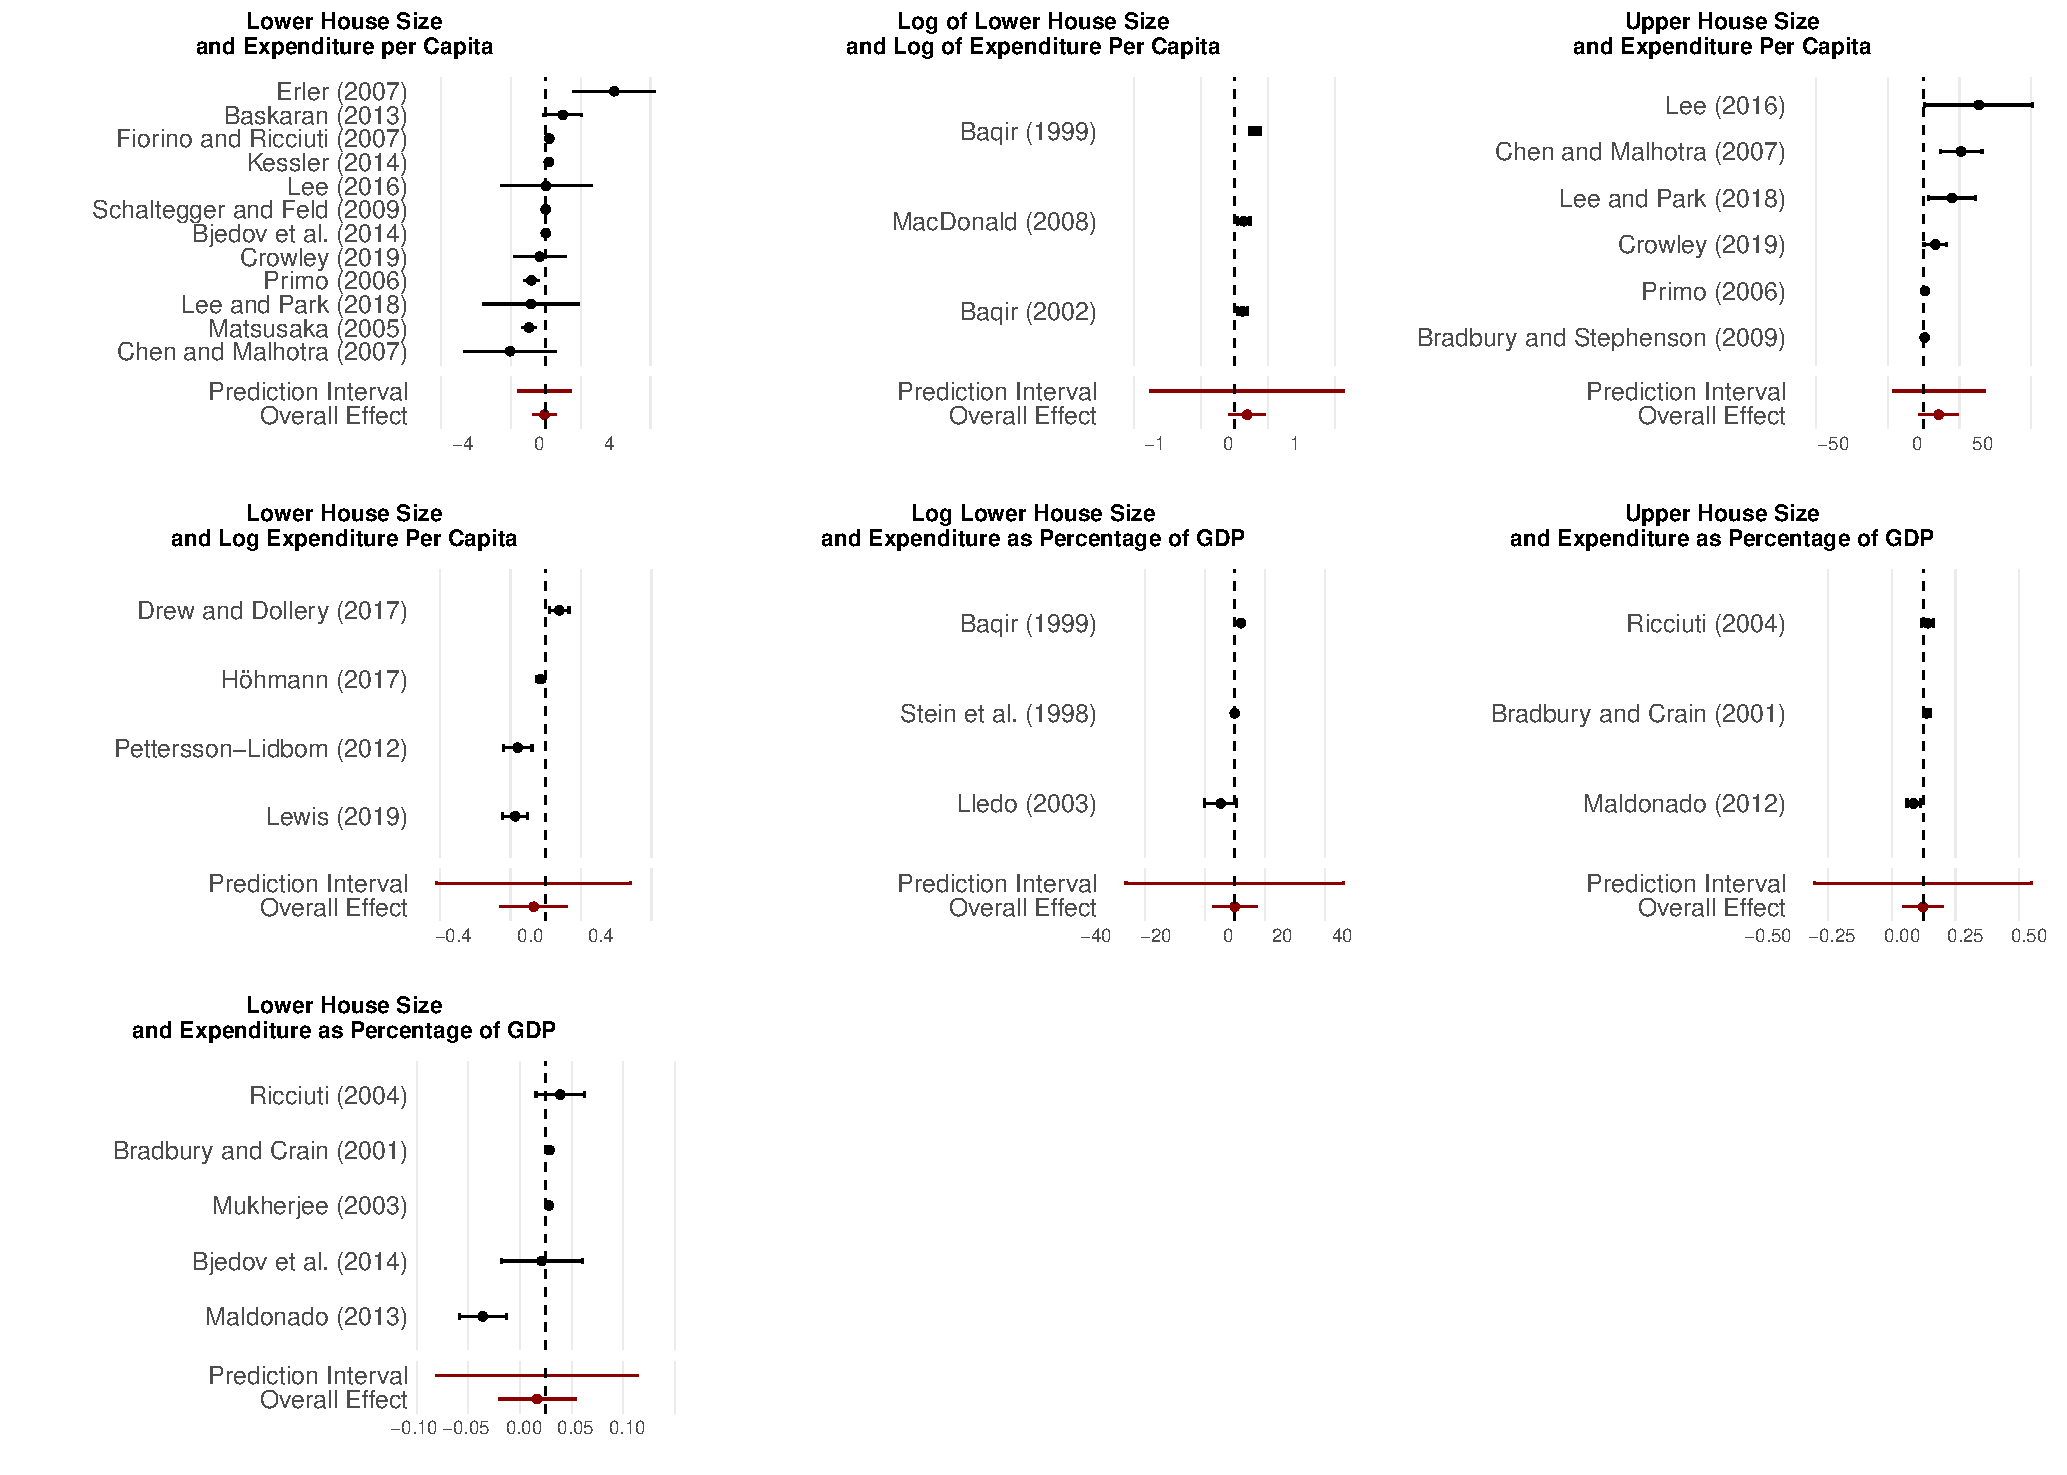
\includegraphics[width=25cm,height=17cm]{meta-analysis.pdf}
\label{fig:plots}
\end{center}
\end{figure}
\end{landscape}

Next, we present the meta-analyses using log($n$), the logarithm of lower house
size, as the main explanatory variable. We start with the relationship between
log($n$) and the logarithm of expenditure per capita. The result is positive and
statistically significant at 10\%, but the prediction interval encompasses zero
(studies = 3, SMD = 0.184, SE = 0.06, 95\% CI = [-0.0738; 0.4425], $p$-value =
0.0916, prediction interval = [-1.258; 1.627], $I^2$ = 85.9\%). Although the
coefficient has the predicted sign, we should interpret the finding with caution
as it does not replicate in our sample of 126 effect sizes.

Our model that correlates log($n$) with public expenditures as a percentage of
GDP fails to reach conventional levels of statistical significance (studies =
3, SMD = 0.0203, SE = 1.677, 95\% CI = [-7.196; 7.237], $p$-value = 0.991,
prediction interval = [-36.206; 36.246], $I^2$ = 96.1\%). The extended sample
also gives us a null result.

The third set of models uses $k$, upper house size, as the main independent
variable. We find a positive correlation between $k$ and expenditure per capita
and the coefficient is significant at a 10\% level (studies = 6, SMD = 10.613, SE
= 5.148, 95\% CI = [-2.621; 23.848], $p$-value = 0.094, prediction interval =
[-21.130; 42.357], $I^2$ = 79.4\%). But as with the other models, the prediction
interval again includes zero. When we run the same analysis in the extended
sample, we also see a significant coefficient yet a prediction interval that
contains zero (coefficients = 24, SMD = 7.216, SE = 1.342, 95\% CI = [4.440; 9.992],
$p$-value $<$ 0.0001, prediction interval = [-1.222; 15.654], $I^2$ = 77.7\%).

Our last estimation analyses the relationship between $k$ and government
spending as a percentage of GDP. The coefficient is not statistically
significant, indicating a null effect (studies = 3, SMD = -0.003, SE =, 95\% CI
= [-0.079; 0.074], $p$-value = 0.891, prediction interval = [-0.428; 0.423],
$I^2$ = 85.8\%). The result is very similar in the extended sample.

In a nutshell, we find only weak evidence in favour of the ``law of $1/n$''.
While some models do show a positive and statistically significant result, none
of the prediction intervals are totally positive or negative. The studies also
have considerable heterogeneity, what indicates that the original coefficients
do not point consistently towards the same direction.

\subsection{Meta-Regressions}
\label{sub:regressions}

In this section, we run a series of meta-regressions with 5 covariates that may
account for differences across the selected papers. The first variable indicates
whether the study uses $n$, log($n$) or $k$ as its main explanatory variable.
The second variable shows the study publication year, which we included to
capture temporal variation in the study coefficients. We also add a dummy
variable to assess whether published articles report effect sizes that are
higher or lower than those from working papers. The fourth variable measures
whether studies focusing on non-majoritarian electoral systems report
coefficients that are smaller or larger than those from majoritarian countries.
Our last covariate is a categorical variable indicating the statistical
procedure used in the original models (panel data, instrumental variables,
OLS, or regression discontinuity design).

Table \ref{tab:regressions} presents the meta-regression results for our
restricted and extended samples. Each column represents one of the three
measures of public spending we discuss in this paper. To reduce the risk of
false positives in our analyses, we use permutation tests to calculate
significance levels for the meta-regressions \citep{higgins2004controlling}.

\vspace{.5cm}

\begin{table}[htpb]
\footnotesize
\caption{Meta Regression Results}
\label{tab:regressions}
\centering
\begin{tabular}{lcccccc}
\toprule
\midrule
\multicolumn{1}{c}{ } & \multicolumn{2}{c}{Expenditure Per Capita} & \multicolumn{2}{c}{Log Expenditure Per Capita} & \multicolumn{2}{c}{Gov. Spending \% GDP} \\
\cmidrule(l{3pt}r{3pt}){2-3} \cmidrule(l{3pt}r{3pt}){4-5} \cmidrule(l{3pt}r{3pt}){6-7}
& Restricted & Extended & Restricted & Extended & Restricted & Extended \\
\midrule
Independent Variable: $N$ & -2.307 & -5.347 &  -0.280 &  -0.0577 &-0.009 & 0.003\\
                          & (1.490)$\dagger$ & (0.929)*** & (0.162) & (0.073) & (0.005)$\dagger$ & (0.005)\\
%
Independent Variable: log($N$) &  &  &  &  &-0.011& 0.002\\
                               &  &  &  &  & (0.001) & (0.014)\\
%
Year & 0.059 & 0.152 &  0.004 &  0.004 &-0.000& -0.000\\
     & (0.101) & (0.078)* & (0.013) & (0.006) & (0.001) & (0.001)\\
%
Published: No &  &  & 0.200 &  0.103 & 0.0625 & 0.060\\
              &  &  & (0.127) & (0.065) & (0.014)* & (0.016)*\\
%
Non-Majoritarian (PR \& Mixed) & 0.428 & 0.985 & &  & -2.055 & -2.169\\
                               & (0.827) & (0.723)$\dagger$ & &  & (0.283)** & (0.166)***\\
%
Method: Panel & 1.203 & -0.135 & 0.188 & -0.252 & 0.055 & 0.058\\
              & (1.575) & (0.797) & (0.093) & (0.068)*** & (0.013)* & (0.017)*\\
%
Method: IV & 1.317 & 0.186 &  &  &  & \\
           & (1.807) & (0.802) &  &  &  & \\
%
Method: RDD &  &  &  &-0.285&  & \\
            &  &  &  & (0.062)*** &  & \\
% 
Intercept & -117.987 & -300.789 & -7.363 & -8.296 & 2.851 & 2.507\\
          & (203.717) & (157.555)* & (25.458) & (12.037) & (1.778) & (2.467)$\dagger$\\
\bottomrule
\end{tabular}
\begin{minipage}{\textwidth}
\renewcommand{\footnoterule}{}
\footnotetext{\textbf{Note:} {The restricted and extended samples include 36 and 126 study coefficients, respectively. We report the results from the permutation tests. Reference categories: Independent Variable $= k$; Published $= Yes$; Non-Majoritarian (PR \& Mixed) $= Majoritarian$; Method $= OLS$. Significance codes: *** $p < 0.001$; ** $p < 0.01$; * $p < 0.05$; $\dagger$ $p < 0.1$.}}
\end{minipage}
\end{table}

The first two models show the results for public expenditure per capita. In both
the restricted and the extended samples, we find that models that use $n$ as an
independent variable tend to detect significantly smaller effects when compared
to $k$. This suggests that an additional member in the lower house has a smaller
impact on public spending than a member in the upper house. Moreover, the
results for the extended sample point out that recent studies find larger
effects than older ones, and that changing the electoral rules from majoritarian
to non-majoritarian increases the effects of legislature size on per capita
expenditure.

The third and fourth columns use the logarithm of expenditure per capita as the
dependent variable. No covariate is statistically significant in our smaller
sample, but two moderators are negatively associated with the outcome in our
larger study pool. They both refer to estimation methods. Studies that employ
panel/fixed effects or regression discontinuity designs (RDDs) have lower
coefficients for log expenditure per capita if we take OLS as the reference
category.

Several variables are statistically significant in the last set of
meta-regressions. The dependent variable is public expenditures as a percentage
of GDP. In our restricted sample, we see that studies with $n$ as an
independent variable have lower coefficients than those that analyse $k$, what
is consistent with our previous models. Both models also show that unpublished
papers tend to have higher coefficients than published papers. Regarding the
electoral systems, see that passing from majoritarian to non-majoritarian
decrease overall levels of public spending. Finally, we find that models
estimated with panel data have larger values than those modelled with OLS.

Overall, our results suggest that study coefficients are highly sensitive to
research design choices. The same statistical methods or study samples may
produce different outcomes depending on the response variables scholars decide
to analyse. Moreover, we find evidence that results vary considerably if the
study employs different measures of legislature size. The impact of factors such
as the electoral system or year of publication also appear to be conditional on
the selected model.

\section{Discussion}
\label{sec:discussion}

In this article, we assess the empirical validity of the ``law of $1/n$''. Based
on a sample of 26 recent publications on the topic, our meta-analyses show that
there is little evidence that an increase in the number of legislators has a
significant effect on public expenditures. If such effect exists, it is likely
driven by an increase in $k$, the size of the upper legislature, as suggested by
several studies in the literature \citep[e.g.,][]{baqir2002districting, 
bradbury2001legislative, bradbury2003local, chen_malhotra_2007,
gilligan2001fiscal, primo2006stop}. We find no robust evidence for the ``reverse
law of $1/n$'', which posits that larger legislatures lead to lower government
spending. One possible explanation is that the two logics are balancing each
other, thus leading us to a null impact of legislature size on public
expenditure.

The meta-regressions indicate that study characteristics have a large influence
on reported results. It is unclear whether factors such as the electoral system
or the level of data aggregation, both believed to moderate the relationship
between legislature size and public expenditure \citep{primo2008distributive,
baqir2002districting, bradbury2003local}, have a substantial impact on the
estimates. We find conflicting evidence for the former and no support for the
latter. Moreover, different statistical techniques produce distinctive results,
which authors should bear in mind.

Our analyses suggest three areas for further research. First, our study sample
did not include articles that evaluate the association between the log($n$) and
public expenditure per capita or between $k$ and log expenditure per capita.
New work on that area might clarify some of the inconsistencies we find
here. Second, despite the inclusion of several moderators in our models,
aggregate results still show considerable heterogeneity. That is, much of the
disparities among studies are yet to be explained. Domestic factors such as
party dynamics or gerrymandering \citep{lee2015supermajority,
mukherjee2003politicalparties, gilligan2006public} may prove useful in this
regard. Finally, we highlight the need for more evidence in favour or against
the ``law of $1/n$'' to inform general public policies. The available empirical
evidence points out that contextual variables may either amplify or reduce the
impact of larger legislatures on government budgets. They should be taken into
account if policy-makers want to reach an optimal balance between sound fiscal
policy and the demands for increased political representation.

\newpage
\bibliography{references.bib}
\bibliographystyle{apalike}

\nocite{baskaran2013coalition, bradbury2009spatially, drew2017price,
erler2007termlimits, fiorino2007legislature, hohmann2017effect,
kessler2014communication, lewis2019legislature, lledo2003electoral,
mukherjee2003politicalparties, petterssonlidbom2012size, schaltegger2009large,
stein1998institutional, mukherjee2003politicalparties, macdonald2008impact,
matsusaka2005endogeneity, ricciuti2004legislatures}

\end{document}
